\documentclass{standalone}
\usepackage{tikz}
\usetikzlibrary{calc}     % 坐标计算库

\begin{document}
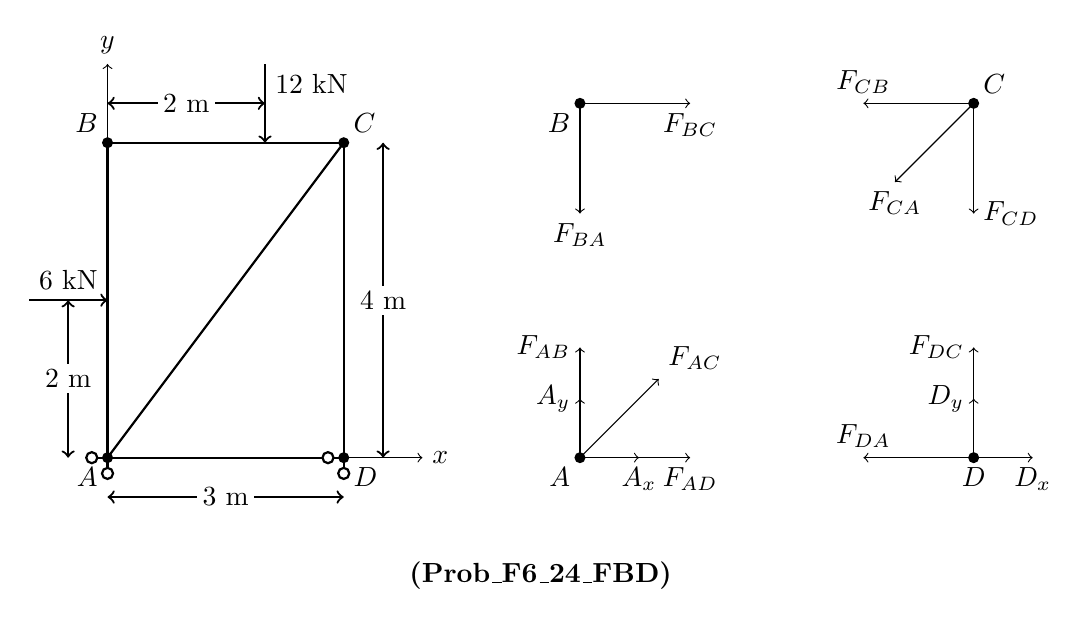
\begin{tikzpicture}

    % 第一个图形,使用 scope 包裹
    \begin{scope}
        % 绘制坐标轴
        \draw[->] (0,0) -- (4,0) node[right] {$x$};
        \draw[->] (0,0) -- (0,5) node[above] {$y$};

        % 绘制点
        \coordinate (A) at (0,0);
        \coordinate (B) at (0,4);
        \coordinate (C) at (3,4);
        \coordinate (D) at (3,0);

        % 填充点
        \fill[black] (A) circle (2pt) node[below left] {$A$};
        \fill[black] (B) circle (2pt) node[above left] {$B$};
        \fill[black] (C) circle (2pt) node[above right] {$C$};
        \fill[black] (D) circle (2pt) node[below right] {$D$};

        % 绘制线段
        \draw[thick] (A) -- (B) -- (C) -- (D) -- cycle;
        \draw[thick] (A) -- (C);

        % 绘制支座 A 点和 D 点
        \draw[thick] (A) -- ++(0,-0.2);
        \draw[thick, fill=white] ($(A) + (0,-0.2)$) circle (2pt);
        \draw[thick] (A) -- ++(-0.2,0);
        \draw[thick, fill=white] ($(A) + (-0.2,0)$) circle (2pt);
        \draw[thick] (D) -- ++(0,-0.2);
        \draw[thick, fill=white] ($(D) + (0,-0.2)$) circle (2pt);
        \draw[thick] (D) -- ++(-0.2,0);
        \draw[thick, fill=white] ($(D) + (-0.2,0)$) circle (2pt);

        % 绘制长度标注
        \draw[thick, <->] ($(A) + (0,-0.5)$) -- ($(D) + (0,-0.5)$);
        \node[fill=white, inner sep=2pt] at ($(A)!0.5!(D) + (0,-0.5)$) {3 m};
        \draw[thick, <->] ($(C) + (0.5,0)$) -- ($(D) + (0.5,0)$);
        \node[fill=white, inner sep=2pt] at ($(C)!0.5!(D) + (0.5,0)$) {4 m};
        \draw[thick, <->] ($(A) + (-0.5,0)$) -- ($(0,2) + (-0.5,0)$);
        \node[fill=white, inner sep=2pt] at ($(A)!0.5!(0,2) + (-0.5,0)$) {2 m};
        \draw[thick, <->] ($(B) + (0,0.5)$) -- ($(2,4) + (0,0.5)$);
        \node[fill=white, inner sep=2pt] at ($(B)!0.5!(2,4) + (0,0.5)$) {2 m};

        % 绘制力
        \draw[<-, thick] (0,2) -- (-1,2) node[above right] {6 kN};
        \draw[<-, thick] (2,4) -- (2,5) node[below right] {12 kN};
    \end{scope}

    % 第二个图形,A
    \begin{scope}[xshift=6cm]
        \coordinate (A) at (0,0);
        \fill[black] (A) circle (2pt) node[below left] {$A$};
        \draw[->] (0,0) -- (0.75,0) node[below] {$A_x$};
        \draw[->] (0,0) -- (0,0.75) node[left] {$A_y$};
        \draw[->] (0,0) -- (1.4,0) node[below] {$F_{AD}$};
        \draw[->] (0,0) -- (0,1.4) node[left] {$F_{AB}$};
        \draw[->] (0,0) -- (1,1) node[above right] {$F_{AC}$};
        % % 绘制逆时针力矩箭头
        % \draw[->] (0,0.3) arc (90:360:0.3) node[above left,xshift=-0.5cm] {$M_1$};
    \end{scope}

    % 第三个图形,B
    \begin{scope}[xshift=6cm,yshift=4.5cm]
        \coordinate (B) at (0,0);
        \fill[black] (B) circle (2pt) node[below left] {$B$};
        \draw[->] (0,0) -- (0,-1.4) node[below] {$F_{BA}$};
        \draw[->] (0,0) -- (1.4,0) node[below] {$F_{BC}$};        
        % % 绘制逆时针力矩箭头
        % \draw[->] (0,0.3) arc (90:360:0.3) node[above, xshift=0.5cm] {$M_2+M_3$};
    \end{scope}

    % 第四个图形,C
    \begin{scope}[xshift=11cm,yshift=4.5cm]
        \coordinate (C) at (0,0);
        \fill[black] (C) circle (2pt) node[above right] {$C$};
        \draw[->] (0,0) -- (-1.4,0) node[above] {$F_{CB}$};
        \draw[->] (0,0) -- (0,-1.4) node[right] {$F_{CD}$};
        \draw[->] (0,0) -- (-1,-1) node[below] {$F_{CA}$};
        % % 绘制逆时针力矩箭头
        % \draw[->] (0,0.3) arc (90:360:0.3) node[below right] {$M_4$};
    \end{scope}

    % 第五个图形,D
    \begin{scope}[xshift=11cm]
        \coordinate (D) at (0,0);
        \fill[black] (D) circle (2pt) node[below] {$D$};
        \draw[->] (0,0) -- (0.75,0) node[below] {$D_x$};
        \draw[->] (0,0) -- (0,0.75) node[left] {$D_y$};
        \draw[->] (0,0) -- (-1.4,0) node[above] {$F_{DA}$};
        \draw[->] (0,0) -- (0,1.4) node[left] {$F_{DC}$};
    \end{scope}

    % 图片标题
    \node[xshift=5.5cm, yshift=-1.5cm] {\textbf{(Prob\_F6\_24\_FBD)}};

\end{tikzpicture}
\end{document}
